\chapter{Uniform Circular Motion and Centripetal Force}


% authors note: verified against AP Phys C 19th edition chapter 13
A Ferris wheel, a spinning washing machine, a car rounding a curve, the
Moon going around Earth: circles are everywhere. So far, you have studied
motion with position, velocity, acceleration, and force mostly along
straight lines and parabolas. What changes when an object moves in a
circle? Surprisingly, it turns out to be accelerating even when its speed
never changes.
\section{Introduction to Uniform Circular Motion}
You may be surprised to know that we can use equations very similar to
the straight-line kinematics equations to describe circular motion,\index{circular motion!equations} provided you use the correct variables.

The angular displacement, $\theta$, is the angle in \emph{radians} that the object has traveled. The angular velocity, $\omega$, is the rate of change of the angular displacement, and the angular acceleration, $\alpha$, is the rate of change of the angular velocity.


\begin{table}[H]
  \centering
  \begin{tabular}{l l}
    Linear motion                          & Rotational motion                                          \\ \hline
    $v = v_0 + a t$                        & $\omega = \omega_0 + \alpha t$                             \\[4pt]
    $x = x_0 + v_0 t + \tfrac{1}{2} a t^2$ & $\theta = \theta_0 + \omega_0 t + \tfrac{1}{2} \alpha t^2$ \\[4pt]
    $v^2 = v_0^2 + 2a(x - x_0)$            & $\omega^2 = \omega_0^2 + 2\alpha(\theta - \theta_0)$
  \end{tabular}
  \caption{Kinematic equations for linear and rotational motion.}
  \label{tab:kinematics_eqs}
\end{table}

\newterm{Linear velocity}, $v$, is related to angular velocity by the equation:
$$v = r \omega$$

The \index{period}\newterm{Period}, $T$, is the time it takes to complete one full rotation. The \index{frequency}frequency, $f$, is the number of rotations per second. The two are related by:
$$T = \frac{2\pi}{\omega} = \frac{2\pi r}{v}$$
$$f = \frac{1}{T}$$

The \index{centripetal force}\newterm{centripetal force}, usually labelled differently (such as tension or gravity), is given by the equation:
$$F = m r \omega^2 = \frac{m v^2}{r}$$


The \newterm{angular velocity,} $\omega$, measures how fast the angle changes. It is measured in radians per second. Over a time interval $\Delta t$, the average angular velocity is
\[
  \omega_{\text{avg}} = \frac{\Delta\theta}{\Delta t}
\]
and the angular velocity at one instant is this ratio for a very short time interval.

\[
  \omega = 2\pi f = \frac{2\pi}{T}
\]

\index{angular acceleration}Angular acceleration measures how fast the angular velocity changes:
\[
  \alpha_{\text{avg}} = \frac{\Delta\omega}{\Delta t}
\]

Note that all of the kinematic formulas still work as long as you stay in the same relative frame of reference (rotational or linear). You cannot ``mix and match'' the two sets of equations.

You may be asking, ``If the object is moving at a constant speed, why is there acceleration?'' Recall that acceleration is a vector quantity, meaning it has both magnitude and direction. Even though the speed (the magnitude of the velocity) is constant, the direction of the velocity vector is always changing. Since acceleration is the rate of change of velocity, any change in direction means there is acceleration. This acceleration is always directed toward the center of the circle, which is why it is called centripetal (center-seeking) acceleration.

Now that we have established the basic relationships for circular motion, let us apply them to a practical example.
\section{The Flying Billiard Ball}
\index{circular motion}
Let us say you tie a 0.16 kg billiard ball to a long string and begin to swing it around in a circle above your head. The string is 3 meters long and stays horizontal, and the ball returns to where it started every 4 seconds. We will assume the ball moves at a constant speed. If you start your stopwatch as the ball crosses the $x$-axis, the coordinates of the position $(x,y,z)$ of the ball at any time $t$ given by:

$$p(t) = \left[3 \cos{\left( \frac{2 \pi} {4}t\right)}, 3 \sin{ \left( \frac{2 \pi}{4}t\right) }, 2\right]$$

(This assumes that the ball would be going counter-clockwise if viewed
from above. The spot you are standing on is considered the origin $[0, 0, 0]$.)

Notice that the height is a constant --- 2 meters in this
case. That is not very interesting, so we will talk just about the
first two components. Figure \ref{fig:billiardBall} shows a visual of the situation:

% 3sin = 1.267854785222098
% 3cos = 2.71892336110995

\begin{figure}[H]
  \begin{center}
    \begin{tikzpicture}[declare function={angle=25;},bullet/.style={inner
            sep=1pt,fill,draw,circle,solid}, scale=1] % right-sized to match other circle diagrams in this chapter
      % Axis
      \draw[thick,-stealth,black] (-3.2,0)--(3.2,0) node[right] {$x$}; % x axis
      \draw[thick,-stealth,black] (0,-3.2)--(0,3.2) node[left] {$y$}; % y axis
      % Rest
      \draw [dashed, sdkblue] (0,0) circle (3);
      \draw[thick] (0,0) -- (angle:3.0) node [midway, above] {3};
      \draw[sdkblue] (1.05, 0.2) node[right] {$\theta = \frac{2\pi t}{4}\text{ radians}$};
      \draw[-stealth,sdkblue] (1,0) arc (0:angle:1);
      \draw[dashed, black] (2.71892336110995, 1.267854785222098) -- (2.71892336110995, 0)
      node[below] {$3 \cos(\theta)$}; % vertical
      \draw[dashed, black] (2.71892336110995, 1.267854785222098) -- (0, 1.267854785222098)
      node[left] {$3 \sin(\theta)$}; % horizontal
      \filldraw[black] (angle:3.0) circle(4pt);
      \draw[->, thick] (2.71892336110995, 1.267854785222098) --
      (2.71892336110995 - 3 * 0.1267, 1.267854785222098 + 3 * 0.2718);
    \end{tikzpicture}
  \end{center}
  \caption{A diagram of our ball and string scenario.}
  \label{fig:billiardBall}
\end{figure}

In this case, the radius, $r$, is 3 meters. The period, $T$, is 4
seconds. In general, we say that circular motion is given by:

$$p(t) = \left[ r \cos{\frac{2 \pi t}{T}}, r \sin{\frac{2 \pi t}{T}}\right]$$

A common question is ``How fast is it turning right now?''  If you
divide the $2\pi$ radians of a circle by the 4 seconds it takes, you
get the answer ``About 1.57 radians per second.''  This is known as
\index{angular velocity}\newterm{angular velocity} and we typically represent it with the
lowercase Omega: $\omega$. (Yes, it looks a lot like a ``w''.)  To be
precise, in our example, the angular velocity is $\omega = \frac{\pi}{2}$. Note that in this scenario, the angular velocity and linear \emph{speed} are constant. However, the \emph{velocity} vector is not constant; as we will see in the next section, the direction of the velocity vector is always changing.

Notice that this is different from the question ``How fast is it
going? (referring to \newterm{linear velocity})''  This ball is traveling the circumference of $6\pi \approx
  18.85$ meters every 4 seconds. This means the speed of the ball is about
4.71 meters per second.

It is very important to distinguish between angular velocity and linear velocity. Angular velocity is how fast the angle is changing and is referred to by $\omega$, while linear velocity, $v$, is how fast the object is moving along its path. While linear velocity has a constant speed, it has always changing direction. The angular velocity is constant, but the linear velocity is not.

\section{Velocity}
\index{circular motion!velocity}
The velocity of the ball is a vector, and we can find it with two facts about circles.

\textbf{Its size.} The ball travels the circumference $2\pi r$ every period $T$, so its speed is
$\frac{2\pi r}{T} = r\omega$. In our example, that is $3 \cdot \frac{\pi}{2} \approx 4.71$ m/s.

\textbf{Its direction.} At every instant, the ball is moving along the circle, so its velocity is tangent to the
circle. A tangent to a circle is perpendicular to the radius. The radius points in the direction
$[\cos \omega t, \sin \omega t]$. Turning a vector $[a, b]$ by $90^\circ$ counterclockwise gives $[-b, a]$, so
the velocity points in the direction $[-\sin \omega t, \cos \omega t]$.

Putting the size and the direction together, in our example, the velocity of the ball at any time $t$ is given by:

$$v(t) = \left[ -\frac{3 (2\pi)}{4} \sin{\frac{2\pi t}{4}}, \frac{3(2\pi)}{4} \cos{\frac{2\pi t}{4}}, 0 \right]$$

Notice that the velocity vector is perpendicular to the position vector. It has a constant magnitude.

In general, an object traveling in a circle at a constant speed has the velocity vector:

$$v(t) = \left[ -r\omega \sin{\omega t}, r\omega \cos{\omega t}\right]$$

where $t = 0$ is the time that it crosses the $x$ axis. If $\omega$ is
negative, that means the motion would be clockwise when viewed from
above. (When you learn derivatives, you will be able to get this same velocity in one line, by
differentiating each component of the position.)

The magnitude of the velocity vector is $r\omega$. See Figure \ref{fig:billardBallVelocity} for a visual of the velocity vector. Note that the $z$-coordinate is constant, so it does not change at all, and it is eliminated from our vector for simplification.
\begin{figure}[H]
  \begin{center}
    \begin{tikzpicture}[declare function={angle=25;},bullet/.style={inner
            sep=1pt,fill,draw,circle,solid}, scale=1] % right-sized to match other circle diagrams in this chapter
      % Axis
      \draw[thick,-stealth,black] (-3.2,0)--(3.2,0) node[right] {$x$}; % x axis
      \draw[thick,-stealth,black] (0,-3.2)--(0,3.2) node[left] {$y$}; % y axis
      % Rest
      \draw [dashed, sdkblue] (0,0) circle (3);
      \filldraw[black] (angle:3.0) circle(4pt);
      \draw[->, thick] (2.71892336110995, 1.267854785222098) --
      (2.71892336110995 - 0.6 * 1.267, 1.267854785222098 + 0.6 * 2.718) node[right]{$v(t)=\left[ -r\omega \sin{\omega t}, r\omega \cos{\omega t}\right]$};
    \end{tikzpicture}
  \end{center}
  \caption{Velocity vector of the ball in circular motion.}
  \label{fig:billardBallVelocity}
\end{figure}

\begin{Exercise}[title = {A Particle in Motion}, label = particle]
  [This question was originally presented as two multiple-choice problems on the 2012 AP Physics C exam.] The $x$ and $y$ coordinates of a particle as it moves in a circle are given by:
  $$x = 5\cos{\left( 3t \right)}\\
    y = 5\sin{\left( 3t \right)}$$

  What is the radius of the particle's circular path? What is the particle's \textit{speed}? Based on your answers, how long does it take the particle to complete the circular path?
  \vspace{50mm}
\end{Exercise}

\begin{Answer}[ref = particle]
  The radius is 5 m, because the coefficients of both the $x$ and $y$ functions is 5.

  The angle is $3t$, so the angular velocity is $\omega = 3$ radians per second. Using the velocity formula
  from this section, with $r = 5$ and $\omega = 3$:
  $$v_x(t) = -15 \sin{ \left( 3t \right)}, \qquad v_y(t) = 15 \cos{ \left( 3t \right)}$$

  The overall \textit{speed} can be found from the $x$ and $y$ components of the velocity:
  \begin{align*}
    |v| & = \sqrt{v_x^2 + v_y^2}                                                              \\ &= \sqrt{\left[ -15 \sin{ \left( 3t \right) } \right]^2 + \left[ 15 \cos{ \left( 3t \right)} \right]^2} \\
        & = \sqrt{15^2 \left[ \sin{ \left(3t \right)}^2 + \cos{ \left( 3t \right)}^2 \right]} \\ &= \sqrt{15^2} = 15 \frac{m}{s}
  \end{align*}

  Notice that this is the coefficient for both components of the velocity.

  To complete the path, the particle must travel $10\pi \text{ } m$. If the speed is $15 \frac{m}{s}$, then the time it takes is:
  $$t = \frac{d}{v} = \frac{10\pi \text{ } m}{15 \frac{m}{s}} = \frac{2\pi}{3} s \approx 2.09 \text{ } s$$
\end{Answer}

\section{Acceleration}

Acceleration is to velocity what velocity is to position: it is the rate at which the velocity vector
changes. Here is a neat trick for finding it. Draw every velocity vector starting from the same point. The
velocity has the constant size $r\omega$ and turns at the same rate $\omega$ as the ball, so its tip moves
around a circle of radius $r\omega$. That is circular motion again! So we can reuse what we just learned: the
rate of change of a vector that moves in a circle of radius $R$ has size $R\omega$ and points $90^\circ$ ahead
of it. Here $R = r\omega$, so the acceleration has size $r\omega^2$, and turning the velocity direction
$[-\sin \omega t, \cos \omega t]$ by another $90^\circ$ gives $[-\cos \omega t, -\sin \omega t]$:

$$a(t) = \left[-r \omega^2 \cos{\omega t}, -r \omega^2 \sin{\omega t} \right] = -r\omega^2 \left[\cos{\omega t}, \sin{\omega t}\right]$$

Notice that the acceleration vector points \textbf{toward the center} of the
circle it is traveling on. That is, when an object is traveling on a
circle at a constant (uniform) speed (notice that coefficients $r$ and $\omega$ are constant), its only acceleration is toward the center of the circle. The acceleration does not come from the motion itself, it comes from the constantly changing direction. This is known as \newterm{centripetal acceleration}. \index{centripetal ! acceleration}

The magnitude of the acceleration vector is $a_c =r \omega^2$, or more commonly, $a_c = \frac{v^2}{r}$. This gives us the common calculation for whatever force acts as the centripetal force: $F_c = m a_c = \frac{m v^2}{r}$.\footnote{You will see centripetal acceleration noted as $a_c$ or $a_r$, standing for centripetal or radial, respectively. Note that both refer to the same acceleration.}

\begin{figure}[H]
  \begin{center}
    \begin{tikzpicture}[declare function={angle=25;},bullet/.style={inner
            sep=1pt,fill,draw,circle,solid}, scale=1] % right-sized to match other circle diagrams in this chapter
      % Axis
      \draw[thick,-stealth,black] (-3.2,0)--(3.2,0) node[right] {$x$}; % x axis
      \draw[thick,-stealth,black] (0,-3.2)--(0,3.2) node[left] {$y$}; % y axis
      % Rest
      \draw [dashed, sdkblue] (0,0) circle (3);
      \filldraw[black] (angle:3.0) circle(4pt);
      \draw[->, thick] (2.71892336110995, 1.267854785222098) --
      (2.71892336110995 * 0.2 , 1.267854785222098 * 0.2) node[midway, right]{$a(t) = \left[-r \omega^2 \cos{\omega t}, -r \omega^2 \sin{\omega t} \right]$};
    \end{tikzpicture}
  \end{center}
  \caption{Acceleration vector of the particle in circular motion.}
  \label{fig:billardBallAcceleration}
\end{figure}

Let us compare the velocity and acceleration paths from figures \ref{fig:billardBallVelocity} and \ref{fig:billardBallAcceleration}. Notice that the velocity vector is always tangent to the circle, while the acceleration vector is always pointing toward the center of the circle.
\begin{figure}[H]
  \centering
  \begin{subfigure}{0.48\textwidth}
    \centering
    \begin{tikzpicture}[declare function={angle=25;}, bullet/.style={inner sep=1pt,fill,draw,circle,solid}, scale=1]
      % Axes
      \draw[thick,-stealth,black] (-3.2,0)--(3.2,0) node[right] {$x$};
      \draw[thick,-stealth,black] (0,-3.2)--(0,3.2) node[left] {$y$};
      % Circle + point
      \draw [dashed, sdkblue] (0,0) circle (3);
      \filldraw[black] (angle:3.0) circle(4pt);
      % Velocity vector
      \draw[->, thick] (2.71892336110995, 1.267854785222098) --
      (2.71892336110995 - 0.6 * 1.267, 1.267854785222098 + 0.6 * 2.718);
      % node[right]{$v(t)=\left[-r\omega \sin(\omega t),\, r\omega \cos(\omega t)\right]$};
    \end{tikzpicture}
    \caption{Velocity vector.}
  \end{subfigure}\hfill
  \begin{subfigure}{0.48\textwidth}
    \centering
    \begin{tikzpicture}[declare function={angle=25;}, bullet/.style={inner sep=1pt,fill,draw,circle,solid}, scale=1]
      % Axes
      \draw[thick,-stealth,black] (-3.2,0)--(3.2,0) node[right] {$x$};
      \draw[thick,-stealth,black] (0,-3.2)--(0,3.2) node[left] {$y$};
      % Circle + point
      \draw [dashed, sdkblue] (0,0) circle (3);
      \filldraw[black] (angle:3.0) circle(4pt);
      % Acceleration vector
      \draw[->, thick] (2.71892336110995, 1.267854785222098) --
      (2.71892336110995 * 0.2 , 1.267854785222098 * 0.2);
      % node[midway, right]{$a(t)=\left[-r\omega^2 \cos(\omega t),\, -r\omega^2 \sin(\omega t)\right]$};
    \end{tikzpicture}
    \caption{Acceleration vector.}
  \end{subfigure}
  \caption{Uniform circular motion: velocity (tangent) and acceleration (centripetal).}
  \label{fig:vel_acc_side_by_side}
\end{figure}

\section{Centripetal force}
What would happen if there were no force pulling the ball toward the center of the circle? It would fly off in a straight line, according to Newton's First Law.

The force you are exerting on the string is what causes it to accelerate toward the center of the circle. We call this the \newterm{centripetal force}. It makes sense that the centripetal force and centripetal acceleration are in the same direction, as they are proportional. \index{centripetal ! force}

Recall that $F = m a$. The magnitude of the acceleration is $r \omega^2 = 3 \left(\frac{2 \pi}{4}\right)^2 \approx 7.4 \mathrm{ m/s}^2$. The mass
of the ball is 0.16 kg. So, the force pulling against your hand is about 1.18 newtons.

The general rule is that when something is traveling in a circle at a
constant speed, the centripetal force needed to keep it traveling in a
circle is:

$$F = m r \omega^2$$

If you know the radius $r$ and the speed $v$ of the object, here is the rule:

$$F = \frac{m v^2}{r}$$

We did not introduce centripetal force as a type of force because it is not its own force, like friction or gravity. Rather, calling a force ``centripetal'' tells us what the force is doing. A centripetal force is any force that causes circular motion, a force which acts in the \emph{radial} direction. For a satellite, the centripetal force is gravity. In the opening example with the billiard ball, the centripetal force is the tension in the string.

\textbf{Example}: A child is sitting on a merry-go-round as it spins. What provides the centripetal force?

\textbf{Solution}: In this case, the child is rotating horizontally, so the centripetal force must also be horizontal. Therefore, the centripetal force is not the child's weight or the normal force. It is the \textit{friction} between the child and the merry-go-round that keeps the child turning. Here is a free body diagram:

\begin{figure}[H]
  \centering
  \begin{tikzpicture}
    \filldraw (0,0) circle (0.12);

    \draw[->] (0,0) -- (0,-2) node[midway,above] {$F_g$};

    \draw[->] (0,0) -- (0,2) node[midway,left] {$F_N$};
    \draw[->] (0,0) -- (3.5,0) node[midway,above] {$F_\text{friction, static}$};
  \end{tikzpicture}
  \caption{The static friction is what causes the centripetal force.}
  \label{fig:merrygoround_fbd}
\end{figure}


\textbf{Example}: If the child is 1.2 meters from the center of the merry-go-round and it spins at 0.25 rotations/second, what is the coefficient of friction between the child and the merry-go-round?

\textbf{Solution}: Using our FBD and applying Newton's Second Law, we see that:
$$F_N - F_g = 0 \to F_N = m_{child}g$$
$$F_f = m r \omega^2 = \mu F_N = \mu m g$$

Since the child is not accelerating vertically, we know that the normal force equals the child's weight. The horizontal force, friction, must equal the mass of the child times the acceleration. Additionally, from the vertical component, we know the friction is equal to $\mu m g$, since the normal force is equal to the child's weight. Looking at the second equation, we see that:
$$m r \omega^2 = \mu m g$$

We were given $\omega$ in rotations per second, but we need radians per second:
$$\frac{0.25 \text{rotation}}{1 \text{second}} = \frac{1 \text{rotation}}{4 \text{seconds}} = \frac{2\pi \text{radians}}{4 \text{seconds}} = \frac{\pi}{2} \frac{rad}{s}$$
We can divide $m$ from both sides of $mr\omega^2 = \mu m g$ (notice: we do not need to know the child's mass to determine the coefficient of friction!):
$$r \omega^2 = \mu g \to \mu = \frac{r \omega^2}{g} = \frac{\left( 1.2 m \right) \left( \frac{\pi}{2 s} \right)^2}{9.8 \frac{m}{s^2}} = 0.302$$

Therefore, the coefficient of friction between the child and the merry-go-round is 0.302.

\subsection{Banked Turns}\index{banked turn}
\begin{wrapfigure}{r}{.65in}
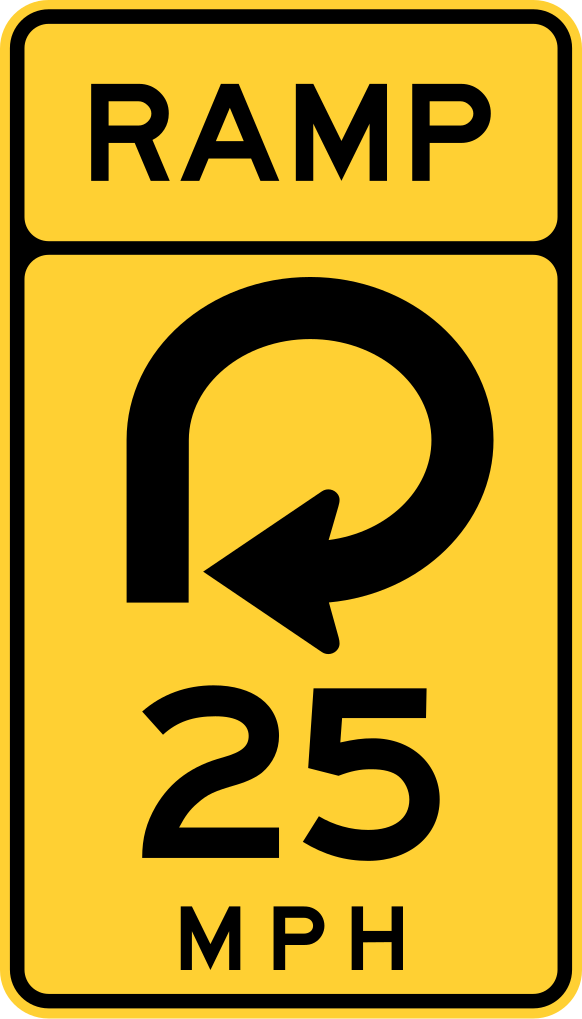
\includegraphics[width=.65in]{traffic.png}
\caption{A banked turn sign.}
\label{fig:traffic}
\end{wrapfigure}
Have you ever been driving on the highway and taken a turn where the road is at an angle? Or maybe you have seen a sign like Figure~\ref{fig:traffic} on the road as you take a turn.


A banked curve is designed so that a car can safely turn without slipping, even in the rain, if the driver does not exceed the indicated speed. Engineers choose an angle such that the bank provides sufficient force to turn the car without friction. Let us look at a free body diagram for a car taking a banked turn (see figure \ref{fig:banked}).

In the past, we have split the vector for the force of gravity into components that are parallel and perpendicular to the ramp. This time, we will split the normal force into $x$ and $y$ components (see figure \ref{fig:banked_component}).

\begin{figure}[H]
  \centering
  \begin{tikzpicture}[scale=0.7]
    \pgfmathsetmacro{\bankangle}{25}
    \pgfmathsetmacro{\rampLen}{9}
    \pgfmathsetmacro{\rampTopY}{\rampLen*tan(\bankangle)}
    \pgfmathsetmacro{\Qx}{5*cos(\bankangle)}
    \pgfmathsetmacro{\Qy}{5*sin(\bankangle)}
    \pgfmathsetmacro{\Px}{\Qx+0.6*cos(\bankangle+90)}
    \pgfmathsetmacro{\Py}{\Qy+0.6*sin(\bankangle+90)}

    % Banked road surface
    \fill[gray!50] (0,0) -- (\rampLen,0) -- (\rampLen,\rampTopY) -- cycle;
    \draw[thick] (0,0) -- (\rampLen,\rampTopY);

    % Bank angle
    \draw (1,0) arc (0:\bankangle:1);
    \node at ({0.5*\bankangle}:1.4) {$\theta$};

    % Car body, wheels, and normal force -- all tilted with the incline
    \begin{scope}[shift={(\Px,\Py)},rotate=\bankangle]
      \draw[fill=sdkblue] (-1.5,-0.3) -- (-1.5,0.05) -- (-0.7,0.05) -- (-0.5,0.35) -- (0.5,0.35) -- (0.6,0.05) -- (1.5,0.05) -- (1.5,-0.3) -- cycle;
      \fill[black] (-1.0,-0.6) rectangle (-0.75,-0.3);
      \fill[black] (0.75,-0.6) rectangle (1.0,-0.3);
      \draw[->] (0,0) -- (0,2.3) node[above] {$F_N$};
      \filldraw[black] (0,0) circle (0.06);
    \end{scope}

    % Gravity always points straight down, regardless of the incline
    \draw[->] (\Px,\Py) -- ++(0,-2.3) node[below] {$F_g$};
  \end{tikzpicture}
  \caption{If there is no friction due to rain, then the only two forces acting on the car are gravity and the normal force.}
  \label{fig:banked}
\end{figure}

Assuming the radius of the turn is 20 m, at what angle should the engineers build the banked turn? (Let us also assume the maximum speed is 25 mph, like the traffic sign above.) First, let us apply Newton's Second Law in the $x$ and $y$ directions:
$$\left( 1 \right) F_N \cos{ \left( \theta \right) } - F_g = 0$$
$$\left( 2 \right) F_N \sin{ \left( \theta \right) } = \frac{mv^2}{r}$$
\begin{wrapfigure}{l}{3.2in}
  \centering
  \begin{tikzpicture}[scale=0.7]
    \pgfmathsetmacro{\bankangle}{25}
    \pgfmathsetmacro{\rampLen}{10}
    \pgfmathsetmacro{\rampTopY}{\rampLen*tan(\bankangle)}
    \pgfmathsetmacro{\Qx}{6.5*cos(\bankangle)}
    \pgfmathsetmacro{\Qy}{6.5*sin(\bankangle)}
    \pgfmathsetmacro{\Px}{\Qx+0.6*cos(\bankangle+90)}
    \pgfmathsetmacro{\Py}{\Qy+0.6*sin(\bankangle+90)}
    \pgfmathsetmacro{\FNlen}{2.8}
    \pgfmathsetmacro{\FNtipX}{\Px+\FNlen*cos(90+\bankangle)}
    \pgfmathsetmacro{\FNtipY}{\Py+\FNlen*sin(90+\bankangle)}
    \pgfmathsetmacro{\FNylen}{\FNlen*cos(\bankangle)}
    \pgfmathsetmacro{\FNxlen}{\FNlen*sin(\bankangle)}
    \pgfmathsetmacro{\dashLen}{\FNlen+0.4}

    % Banked road surface
    \fill[gray!50] (0,0) -- (\rampLen,0) -- (\rampLen,\rampTopY) -- cycle;
    \draw[thick] (0,0) -- (\rampLen,\rampTopY);

    % Bank angle at the base
    \draw (1,0) arc (0:\bankangle:1);
    \node at ({0.5*\bankangle}:1.4) {$\theta$};

    % Car body and wheels -- tilted with the incline
    \begin{scope}[shift={(\Px,\Py)},rotate=\bankangle]
      \draw[fill=sdkblue] (-1.5,-0.3) -- (-1.5,0.05) -- (-0.7,0.05) -- (-0.5,0.35) -- (0.5,0.35) -- (0.6,0.05) -- (1.5,0.05) -- (1.5,-0.3) -- cycle;
      \fill[black] (-1.0,-0.6) rectangle (-0.75,-0.3);
      \fill[black] (0.75,-0.6) rectangle (1.0,-0.3);
      \filldraw[black] (0,0) circle (0.06);
    \end{scope}

    % Normal force, perpendicular to the ramp
    \draw[->,thick] (\Px,\Py) -- (\FNtipX,\FNtipY) node[above left] {$F_N$};

    % Gravity, straight down
    \draw[->,thick] (\Px,\Py) -- ++(0,-2.2) node[below] {$F_g$};

    % Vertical reference (dashed)
    \draw[dashed] (\Px,\Py) -- ++(0,\dashLen);

    % Components of F_N
    \draw[->,red!70!black,thick] (\Px,\Py) -- ++(0,\FNylen) node[right,align=left] {$F_{N,y} =$\\$F_N\cos(\theta)$};
    \draw[->,red!70!black,thick] (\Px,\Py) -- ++(-\FNxlen,0) node[left,align=left] {$F_{N,x} =$\\$F_N\sin(\theta)$};

    % Angle between vertical reference and F_N
    \pgfmathsetmacro{\arcR}{1.3}
    \draw (\Px,{\Py+\arcR}) arc (90:{90+\bankangle}:\arcR);
    \pgfmathsetmacro{\arcMid}{90+\bankangle/2}
    \pgfmathsetmacro{\labelR}{1.7}
    \pgfmathsetmacro{\thetaLabelX}{\Px+\labelR*cos(\arcMid)}
    \pgfmathsetmacro{\thetaLabelY}{\Py+\labelR*sin(\arcMid)}
    \node at (\thetaLabelX,\thetaLabelY) {$\theta$};
  \end{tikzpicture}
  \caption{Geometrically, the vertical ($y$) component of the normal force is $F_N \cos{\left( \theta \right)}$ and the horizontal ($x$) component is $F_N \sin{ \left( \theta \right)}$.}
  \label{fig:banked_component}
\end{wrapfigure}

We know that $F_g = mg$. From this and equation (1) we see that:
$$F_N = \frac{mg}{\cos{ \left( \theta \right)}}$$

Substituting for $F_N$ into equation (2):
$$\left( \frac{mg}{\cos{ \left( \theta \right)}} \right) \sin{ \left( \theta \right)} = \frac{mv^2}{r}$$

The mass can be divided from both sides, and $\frac{\sin{ \left( \theta \right)}}{\cos{ \left( \theta \right)}} = \tan{ \left( \theta \right)}$:
$$g \tan{ \left( \theta \right)} = \frac{v^2}{r}$$

Solving for $\theta$ and substituting for the speed ($25 \text{ }mph \approx 11.18 \frac{m}{s}$) and radius:
$$\theta = \arctan{ \left( \frac{v^2}{gr} \right)} = \arctan{ \left( \frac{\left( 11.18 \frac{m}{s} \right)^2}{\left( 9.8 \frac{m}{s^2} \right) \left( 20 m \right)} \right)}$$
$$\theta = \arctan{ \left( 0.6377 \right) } \approx 32.53 ^{\circ}$$

The next chapter, Circular Motion in Action, puts centripetal force to work on swinging objects and roller
coaster loops.
